\chapter{Phương pháp}
\label{Chapter3}
\setcounter{secnumdepth}{5}

\section{Dữ liệu}

Mô hình LViT trong báo cáo này được huấn luyện và kiểm thử trên ba tập dữ liệu y khoa có đi kèm mặt nạ phân đoạn và mô tả tổn thương. Các bộ dữ liệu này khác nhau về loại ảnh, số lượng mẫu và cách xây dựng chú thích văn bản, nhưng đều phục vụ chung cho bài toán phân đoạn tổn thương dựa trên thông tin thị giác và ngôn ngữ.

\subsection{Mô tả các bộ dữ liệu}

\begin{enumerate}
    \item \textbf{QaTa-COV19-v2:}\footnote{\href{https://www.kaggle.com/datasets/aysendegerli/qatacov19-dataset}{https://www.kaggle.com/datasets/aysendegerli/qatacov19-dataset}} bao gồm 9258 ảnh X-ray ngực được ghi chú thủ công các thương tổn do COVID-19. Nhóm nghiên cứu đã mở rộng phần chú thích với sự hỗ trợ của các chuyên gia. Nội dung chú thích tập trung vào tình trạng nhiễm bệnh ở một hoặc hai phổi, số lượng vùng thương tổn và vị trí tương đối của các vùng nhiễm bệnh. Ví dụ: ``Bilateral pulmonary infection, two infected areas, upper left lung and upper right lung'' (tạm dịch: ``Nhiễm trùng phổi hai bên, hai vùng nhiễm bệnh, ở phía trên phổi trái và phía trên phổi phải'').

    \item \textbf{MosMedData+:}\footnote{\href{http://medicalsegmentation.com/covid19}{http://medicalsegmentation.com/covid19}} bao gồm 2729 ảnh CT scan về nhiễm trùng phổi. Cấu trúc chú thích của tập dữ liệu này tương tự QaTa-COV19-v2, bao gồm phạm vi nhiễm bệnh, số vùng tổn thương và vị trí tương đối của vùng nhiễm. Ví dụ: ``Unilateral pulmonary infection, two infected areas, middle lower left lung'' (tạm dịch: ``Nhiễm trùng phổi một bên, hai vùng nhiễm bệnh, ở giữa phía dưới phổi trái'').

    \item \textbf{ESO-CT:} bao gồm 286 ảnh X-ray được ghi chú độc lập bởi hai chuyên gia. Tập dữ liệu này tập trung vào ung thư thực quản và cung cấp thông tin vị trí tổn thương phục vụ cho bài toán phân đoạn.
\end{enumerate}

\subsection{Quy trình xây dựng chú thích văn bản}

Phần ghi chú thông tin bệnh của các bộ dữ liệu không có sẵn ngay từ đầu, mà được nhóm nghiên cứu tạo ra và mở rộng với sự hỗ trợ trực tiếp của hai chuyên gia từ Khoa Xạ trị Ung thư \footnote{Trung tâm Y tế Tây Nam trường Đại học Texas}.

Quy trình tạo và kiểm duyệt chất lượng chú thích được thực hiện chặt chẽ giữa các chuyên gia và nhóm nghiên cứu. Các bác sĩ X-quang tiến hành chú thích độc lập trên cùng một ảnh. Sau đó, kết quả được nhóm nghiên cứu đối chiếu để đảm bảo tính nhất quán, họ cũng kiểm tra chéo các đoạn văn bản này với mặt nạ phân đoạn gốc của ảnh nhằm bảo đảm rằng thông tin vị trí trong văn bản không sai lệch quá lớn so với vùng tổn thương thực tế.

\subsection{Cấu trúc chú thích}

Nội dung và cấu trúc chú thích được thiết kế theo đặc điểm của từng nhóm dữ liệu:

\begin{itemize}
    \item \textbf{QaTa-COV19-v2 và MosMedData+:} Văn bản chú thích được cấu trúc hóa thống nhất, tập trung vào ba thuộc tính chính: phạm vi nhiễm bệnh, số lượng vùng tổn thương và vị trí ước chừng của vùng nhiễm.

    \item \textbf{ESO-CT:} Tập dữ liệu ung thư thực quản bao gồm các thông tin lâm sàng được bác sĩ X-quang chú thích thủ công. Để tạo văn bản mô tả, bác sĩ chia thực quản thành bốn phần từ trên xuống dưới, gồm cổ, ngực trên, ngực giữa và ngực dưới; sau đó ghi chú vị trí ước chừng của khối u dựa trên các phần này. Đoạn văn bản mô tả vị trí thô được sử dụng trực tiếp làm đầu vào cho mô hình.
\end{itemize}

\subsection{Phân chia dữ liệu}

Số lượng mẫu trong từng tập huấn luyện, kiểm định và kiểm thử được chia như sau:

\begin{table}[H]
    \centering
    \begin{tabular}{cccc}
    \hline
    & \textbf{QaTa-COV19-v2} & \textbf{MosMedData+} & \textbf{ESO-CT} \\
    \hline
    Tập huấn luyện & 5716 & 2183 & 182 \\
    Tập kiểm định & 1429 & 273 & 273 \\
    Tập kiểm thử & 2113 & 273 & 58 \\
    \hline
    Tổng cộng & 9528 & 2729 & 286 \\
    \hline
    \end{tabular}
    \caption{Phân phối dữ liệu trong các tập dữ liệu}
\end{table}


% \begin{enumerate}
%     \item QaTa-COV19-v2: Train (5716), Val (1429), Test (2113).
%     \item MosMedData+: Train (2183), Val (273), Test (273).
%     \item ESO-CT: Train (182), Val (46), Test (58).
% \end{enumerate}

\begin{figure}[H]
    \centering
    \begin{minipage}{0.45\linewidth}
        \centering
        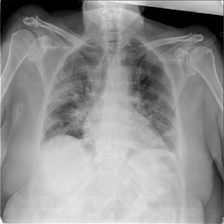
\includegraphics[width=0.7\linewidth]{images/qata-cov19-v2-covid_1.png}

        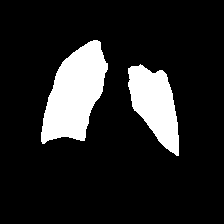
\includegraphics[width=0.7\linewidth]{images/qata-cov19-v2-mask_covid_1.png}

        QaTa-COV19-v2 (224 $\times$ 224)
    \end{minipage}
    \hfill
    \begin{minipage}{0.45\linewidth}
        \centering
        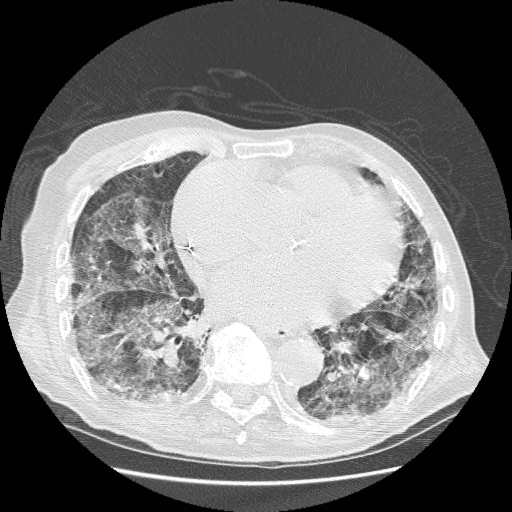
\includegraphics[width=0.7\linewidth]{images/mosmed_bjorke_1.png}

        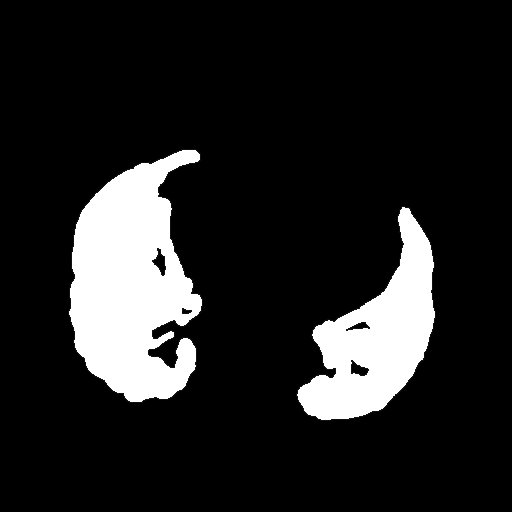
\includegraphics[width=0.7\linewidth]{images/mosmed_mask_bjorke_1.png}

        MosMedData+ (512 $\times$ 512)
    \end{minipage}
    \caption{Ví dụ ảnh đầu vào và mặt nạ phân đoạn trong các bộ dữ liệu.}
\end{figure}

\section{Kiến trúc mô hình}

Mô hình LViT được xây dựng theo hướng kết hợp đặc trưng thị giác và đặc trưng ngôn ngữ nhằm thực hiện phân đoạn ảnh có điều kiện theo câu nhắc văn bản. Kiến trúc tổng quát gồm hai nhánh chính:

\begin{enumerate}
    \item Nhánh CNN U-shape dùng để trích xuất đặc trưng cục bộ và bảo toàn thông tin không gian.
    \item Nhánh ViT U-shape dùng để học quan hệ toàn cục và tích hợp thông tin văn bản vào biểu diễn hình ảnh.
\end{enumerate}

\begin{figure}[H]
    \centering
    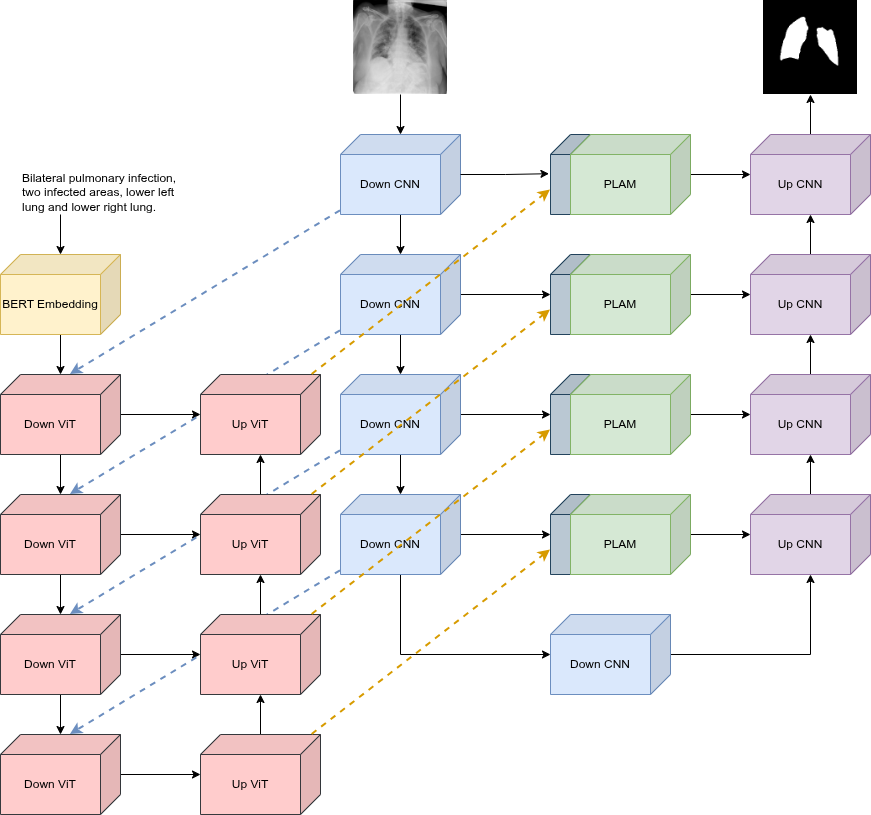
\includegraphics[width=0.7\linewidth]{images/lvit.png}
    \caption{Kiến trúc mô hình LViT.}
\end{figure}

\begin{figure}[H]
    \centering
    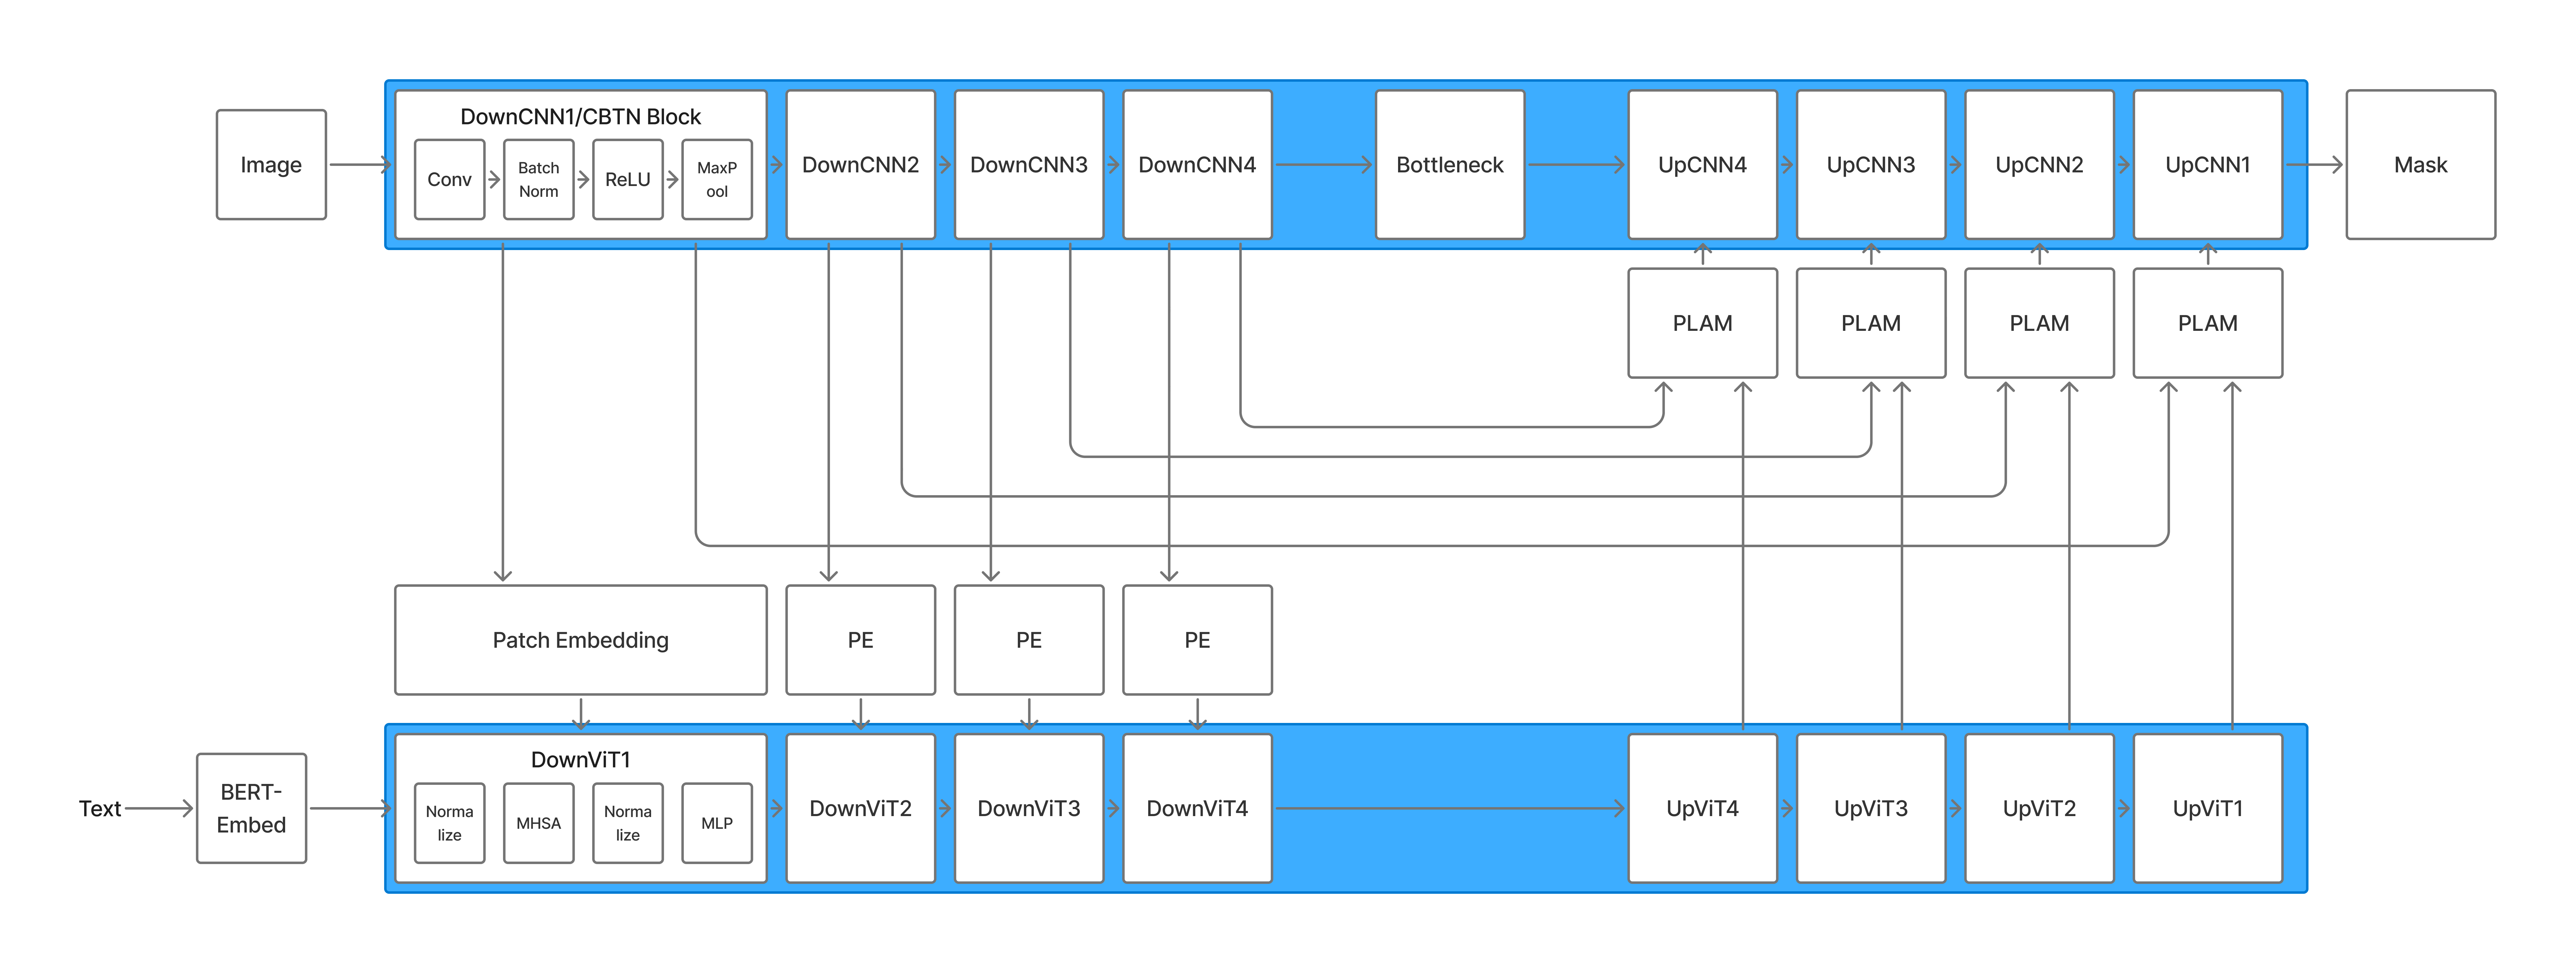
\includegraphics[width=\linewidth]{images/flatten-lvit.png}
    \caption{Minh họa quá trình làm phẳng và xử lý đặc trưng trong LViT.}
\end{figure}

\subsection{Nhánh CNN U-shape}

Nhánh CNN nhận đầu vào là ảnh y khoa và tạo ra các đặc trưng thị giác ở nhiều mức độ phân giải khác nhau. Các khối tích chập giúp mô hình học các đặc trưng cục bộ như biên, kết cấu và hình dạng tổn thương, trong khi các phép giảm mẫu giúp mở rộng vùng tiếp nhận của mô hình. Đồng thời, nhánh CNN cũng đóng vai trò là đầu ra phân đoạn để tạo ra mặt nạ dự đoán xác suất.

\begin{figure}[H]
    \centering
    \begin{minipage}{0.48\linewidth}
        \begin{align*}
            D_i &= DownCNN_i = CTBN \\
                &= ReLU(BatchNorm_i(Conv_i(\cdot)))
        \end{align*}
        \[
            Y_{DownCNN, i+1} = MaxPool(D_i(Y_{DownCNN, i}))
        \]
        \[
            Y_{DownCNN, 0} = I
        \]
    \end{minipage}
    \hfill
    \begin{minipage}{0.42\linewidth}
        \centering
        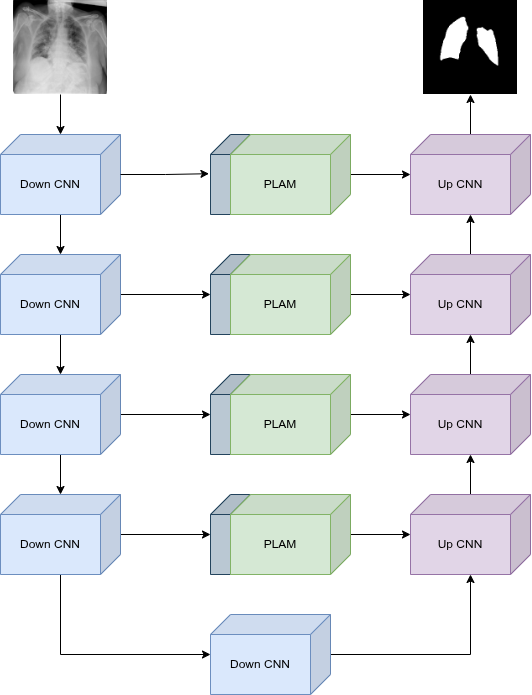
\includegraphics[width=0.85\linewidth]{images/cnn-branch.png}
    \end{minipage}
    \caption{Nhánh CNN U-shape và công thức cập nhật đặc trưng.}
\end{figure}

Trong đó, $Conv_i$ là phép tích chập tại tầng thứ $i$, $BatchNorm_i$ là chuẩn hóa theo batch, $ReLU$ là hàm kích hoạt phi tuyến và $MaxPool$ là phép giảm kích thước không gian. Kết quả của nhánh CNN được sử dụng làm nền tảng cho quá trình mã hóa thị giác và kết hợp với thông tin văn bản ở các bước sau.

Tại các nhánh skip connection, đặc trưng từ UpViT được điều chỉnh về cùng kích thước không gian với đặc trưng từ DownCNN để hai nguồn thông tin có thể được kết hợp trực tiếp. Đặc trưng DownCNN thường chứa nhiều chi tiết cục bộ như biên, kết cấu và vị trí không gian của vùng tổn thương, trong khi đặc trưng UpViT mang nhiều thông tin ngữ nghĩa và ngữ cảnh toàn cục hơn nhờ cơ chế attention. Việc kết hợp hai loại đặc trưng này giúp mô hình vừa giữ được độ chính xác ở mức pixel, vừa tận dụng được khả năng mô hình hóa quan hệ dài hạn của nhánh ViT. Sau bước căn chỉnh kích thước và hợp nhất đặc trưng, kết quả được đưa vào mô-đun PLAM nhằm bảo toàn thông tin cục bộ từ CNN, đồng thời bổ sung ngữ cảnh toàn cục từ nhánh ViT trước khi tiếp tục quá trình giải mã mặt nạ.

\subsection{Nhánh ViT U-shape}

Khối DownViT đầu tiên nhận đầu vào là đặc trưng ảnh từ khối DownCNN thứ nhất, đồng thời kết hợp với đặc trưng văn bản được sinh ra từ lớp BERT-Embed của BERT\_12\_768\_12. Thông qua cơ chế patch embedding, đặc trưng ảnh được chuyển thành các visual token để có thể xử lý bằng Transformer.

\begin{figure}[H]
    \centering
    \begin{minipage}{0.36\linewidth}
        \centering
        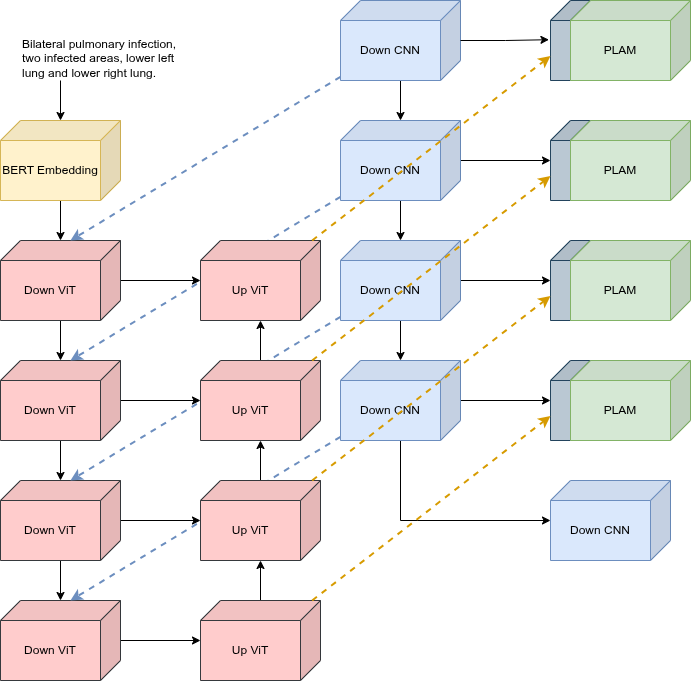
\includegraphics[width=\linewidth]{images/vit-branch.png}
    \end{minipage}
    \hfill
    \begin{minipage}{0.58\linewidth}
        \begin{align*}
            Y_{DownViT, 1} &= ViT(x_{img, 1} + CTBN(x_{text})) \\
            x_{img, i} &= PatchEmbedding(Y_{DownCNN, i}) \\
            x_{text} &= BERT\_Embed (\text{text prompt}) \\ \\
            ViT(x) &= ViT_2(ViT_1(x)) \\
            x' &= ViT_1(x) = MHSA(LN(x)) + x \\
            Y &= ViT_2(x') = MLP(LN(x')) + x' \\
        \end{align*}
    \end{minipage}
    \caption{Nhánh ViT U-shape và quá trình tích hợp đặc trưng ảnh-văn bản.}
\end{figure}

Trong các công thức trên, $LN$ là Layer Normalization. Đặc trưng văn bản $x_{text}$ được chiếu về không gian phù hợp thông qua $CTBN$ trước khi cộng với đặc trưng ảnh, giúp thông tin ngôn ngữ tham gia vào quá trình học biểu diễn thị giác.

Các khối ViT tiếp theo nhận đặc trưng từ khối ViT phía trên và đặc trưng từ khối DownCNN ở mức tương ứng.

\[
    Y_{DownViT, i+1} = ViT(Y_{DownViT, i} + x_{img, i + 1}), \quad i = 1, 2, 3
\]

Tại các khối UpViT, các token ngữ nghĩa được cộng với phần dư tương ứng từ nhánh DownViT nhằm bảo toàn thông tin toàn cục đã được học ở giai đoạn mã hóa. Cơ chế cộng phần dư này giúp đặc trưng ở nhánh giải mã không bị mất các quan hệ dài hạn giữa các vùng ảnh, đồng thời tiếp tục duy trì quá trình tương tác attention giữa các token. Nhờ đó, UpViT không chỉ khôi phục dần độ phân giải không gian mà còn giữ được ngữ cảnh ngữ nghĩa đã được tích hợp từ văn bản. Sau khi đi qua các khối UpViT, đặc trưng được điều chỉnh về kích thước phù hợp để cộng trực tiếp với đặc trưng DownCNN ở cùng mức phân giải. Sự kết hợp này giúp mô hình tận dụng đồng thời thông tin toàn cục từ ViT và chi tiết cục bộ từ CNN trước khi đưa vào mô-đun PLAM để tiếp tục tinh chỉnh đặc trưng phục vụ cho quá trình giải mã mặt nạ.

\subsection{Mô-đun Patch Embedding}
Để kết hợp đặc trưng thị giác từ ảnh với đặc trưng văn bản trong nhánh Transformer, bản đồ đặc trưng hình ảnh cần được chuyển đổi từ dạng không gian hai chiều sang dạng chuỗi token. Ở nhánh CNN, đặc trưng ảnh thường được biểu diễn dưới dạng tensor gồm số kênh, chiều cao và chiều rộng. Trong khi đó, Transformer không xử lý trực tiếp ảnh như một lưới pixel hai chiều, mà tiếp nhận đầu vào dưới dạng một chuỗi các vector đặc trưng. Vì vậy, mô-đun Patch Embedding đóng vai trò trung gian, giúp chuyển đặc trưng ảnh sang định dạng phù hợp với cơ chế attention.

Cụ thể, mô-đun Patch Embedding chia bản đồ đặc trưng ảnh thành nhiều vùng nhỏ gọi là patch. Trong cài đặt thực tế, bước này thường được thực hiện bằng một lớp tích chập với kích thước kernel và stride tương ứng với kích thước patch. Mỗi patch sau khi đi qua phép chiếu sẽ được mã hóa thành một vector đặc trưng, gọi là visual token. Visual token này đại diện cho thông tin thị giác cục bộ của một vùng trong ảnh, chẳng hạn biên tổn thương, kết cấu mô hoặc sự thay đổi cường độ tại vùng bệnh lý.

Sau khi tạo ra các visual token, mô hình ghép chúng lại theo thứ tự không gian để tạo thành một chuỗi token hoàn chỉnh. Tuy nhiên, quá trình chuyển từ bản đồ đặc trưng hai chiều sang chuỗi một chiều có thể làm mất thông tin về vị trí tương đối giữa các patch. Để khắc phục điều này, mỗi visual token được cộng thêm positional embedding. Thành phần này giúp mô hình nhận biết token tương ứng đến từ vùng nào trong ảnh, ví dụ phía trên, phía dưới, bên trái hoặc bên phải. Đây là thông tin đặc biệt quan trọng trong phân đoạn ảnh y khoa, vì vị trí tổn thương thường liên quan trực tiếp đến nội dung mô tả trong câu nhắc văn bản.

Sau bước Patch Embedding, chuỗi visual token được đưa vào các khối attention của nhánh ViT để học quan hệ toàn cục giữa các vùng ảnh. Đồng thời, vì đặc trưng văn bản cũng được biểu diễn dưới dạng các vector token, mô hình có thể đưa thông tin thị giác và ngôn ngữ về cùng một không gian biểu diễn. Nhờ đó, các token hình ảnh không chỉ chứa thông tin về cấu trúc và vị trí của vùng tổn thương, mà còn có thể được điều kiện hóa bởi nội dung mô tả trong văn bản đầu vào.

\subsection{Bộ mã hóa văn bản}

Bộ mã hóa văn bản đóng vai trò chuyển câu mô tả y khoa thành các vector đặc trưng ngữ nghĩa để mô hình có thể sử dụng trong quá trình phân đoạn. Trước hết, câu mô tả được tách thành các token, sau đó mỗi token được ánh xạ sang một vector nhúng thông qua lớp Embedding của BERT. Các vector này chứa thông tin về ý nghĩa của từng thành phần trong câu, chẳng hạn như vị trí tổn thương, số lượng vùng nhiễm bệnh, phạm vi nhiễm bệnh và các đặc điểm mô tả liên quan. Nhờ đó, đặc trưng văn bản có thể đóng vai trò như một tín hiệu điều kiện, giúp nhánh thị giác tập trung vào đúng vùng mục tiêu thay vì chỉ dựa vào đặc trưng hình ảnh thuần túy.

Trong LViT, các câu mô tả y khoa thường có cấu trúc tương đối cố định và ngắn gọn, ví dụ bao gồm phạm vi nhiễm bệnh, số vùng tổn thương và vị trí tương đối. Do đó, mô hình không nhất thiết phải sử dụng toàn bộ các tầng Transformer của BERT để suy luận ngữ cảnh phức tạp như trong các bài toán xử lý ngôn ngữ tự nhiên tổng quát. Thay vào đó, việc sử dụng lớp Embedding của BERT đã đủ để cung cấp biểu diễn ban đầu cho các token văn bản, đồng thời giúp giảm số lượng tham số, tiết kiệm chi phí tính toán và hạn chế nguy cơ quá khớp khi dữ liệu y khoa có quy mô không quá lớn.

\begin{figure}[H]
    \centering
    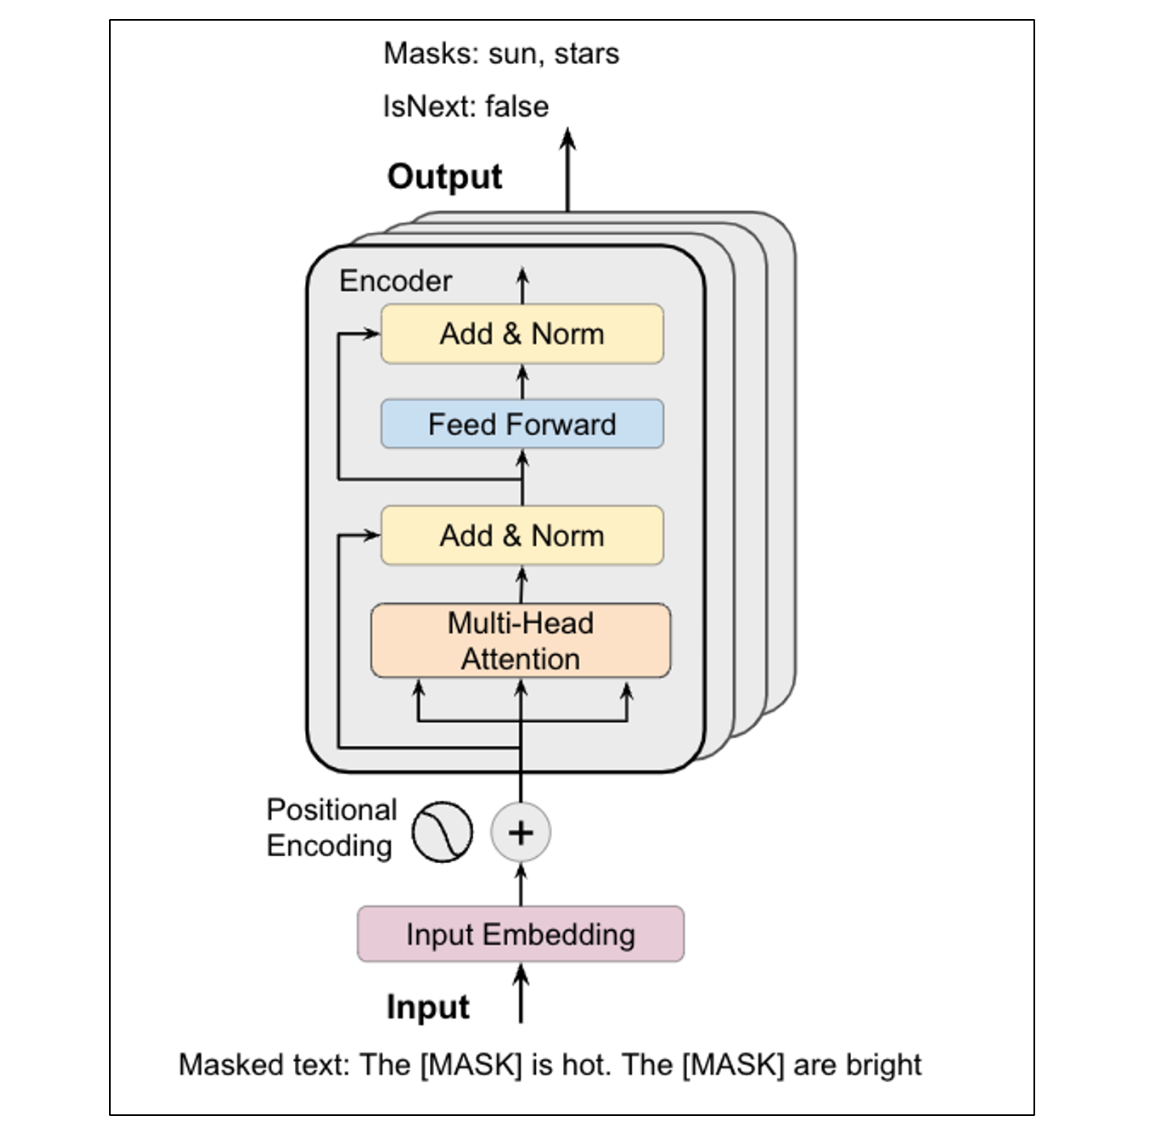
\includegraphics[width=0.7\linewidth]{images/bert.png}
    \caption{Bộ mã hóa văn bản dựa trên BERT.}
\end{figure}

\subsection{Mô-đun Reconstruct}
Sau khi các khối ViT học được quan hệ ngữ nghĩa giữa đặc trưng hình ảnh và đặc trưng văn bản, dữ liệu cần được chuyển trở lại dạng bản đồ đặc trưng để có thể kết hợp với nhánh CNN. Lý do là nhánh ViT biểu diễn dữ liệu dưới dạng chuỗi token, trong đó mỗi token đại diện cho một patch hoặc một vùng đặc trưng của ảnh. Ngược lại, nhánh CNN xử lý dữ liệu dưới dạng tensor không gian hai chiều, gồm số kênh, chiều cao và chiều rộng. Vì vậy, trước khi thực hiện cộng phần dư hoặc nối đặc trưng với nhánh CNN, chuỗi token từ ViT phải được tái cấu trúc thành bản đồ đặc trưng tương thích.

Mô-đun Reconstruct đảm nhiệm quá trình chuyển đổi này. Trước hết, chuỗi token được sắp xếp lại theo thứ tự không gian ban đầu của các patch để tạo thành một lưới hai chiều. Nếu ở bước Patch Embedding, bản đồ đặc trưng được chia thành các patch và làm phẳng thành chuỗi, thì ở bước Reconstruct, quá trình này được thực hiện theo chiều ngược lại: các token được đưa về đúng vị trí tương ứng trên mặt phẳng không gian. Nhờ đó, thông tin toàn cục học được bởi Transformer có thể được biểu diễn lại dưới dạng bản đồ đặc trưng mà CNN có thể xử lý.

Sau khi khôi phục cấu trúc hai chiều, bản đồ đặc trưng thường vẫn có độ phân giải thấp hơn so với đặc trưng ở nhánh CNN tương ứng, vì mỗi token ban đầu chỉ đại diện cho một vùng patch thay vì một pixel riêng lẻ. Do đó, mô-đun Reconstruct cần thực hiện bước tăng kích thước không gian, chẳng hạn bằng nội suy hoặc các thao tác upsampling, để đưa bản đồ đặc trưng về cùng kích thước với nhánh CNN. Bước căn chỉnh này rất quan trọng, vì các phép toán như cộng phần dư hoặc ghép kênh chỉ thực hiện được khi hai tensor có cùng chiều cao và chiều rộng.

Cuối cùng, kết quả sau khi tái cấu trúc và tăng kích thước được đưa qua một lớp tích chập để điều chỉnh số kênh và tinh chỉnh lại biểu diễn đặc trưng. Lớp tích chập này giúp chuyển đặc trưng từ không gian token của ViT sang không gian đặc trưng phù hợp hơn với CNN, đồng thời làm mượt các thông tin sau bước nội suy. Nhờ mô-đun Reconstruct, LViT có thể kết hợp hiệu quả ưu điểm của Transformer trong việc học ngữ cảnh toàn cục với ưu điểm của CNN trong việc giữ chi tiết không gian cục bộ, phục vụ tốt hơn cho quá trình giải mã mặt nạ phân đoạn.

\subsection{Mô-đun PLAM}

Mô-đun PLAM được thiết kế nhằm bảo toàn đặc trưng cục bộ của ảnh, đồng thời tăng cường khả năng khai thác thông tin ngữ nghĩa từ đặc trưng văn bản. Trong kiến trúc LViT, nhánh Transformer có ưu điểm trong việc học các quan hệ toàn cục giữa các vùng ảnh thông qua cơ chế self-attention. Tuy nhiên, do tập trung vào tương tác toàn cục, Transformer có thể làm suy giảm một số chi tiết cục bộ quan trọng như biên tổn thương, kết cấu nhỏ hoặc sự thay đổi cường độ tại các vùng hẹp. Đây là những thông tin có vai trò quan trọng trong phân đoạn ảnh y khoa, đặc biệt khi vùng bệnh lý có kích thước nhỏ hoặc ranh giới không rõ ràng.

\begin{figure}[H]
    \centering
    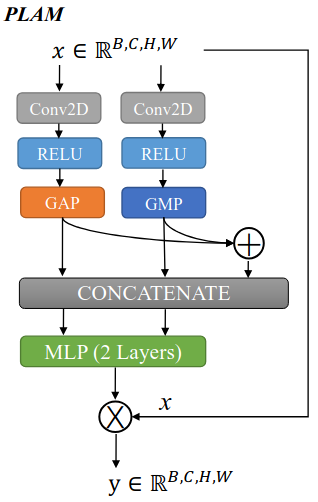
\includegraphics[width=0.5\linewidth]{images/plam.png}
    \caption{Mô-đun PLAM trong kiến trúc LViT.}
\end{figure}

PLAM được đưa vào để bù đắp hạn chế này bằng cách kết hợp thông tin từ nhiều nhánh đặc trưng khác nhau. Cụ thể, mô-đun sử dụng hai nhánh song song gồm Global Average Pooling và Global Max Pooling. Global Average Pooling giúp mô hình nắm bắt xu hướng tổng quát của toàn bộ bản đồ đặc trưng, trong khi Global Max Pooling nhấn mạnh các đặc điểm mạnh nhất, thường tương ứng với những vùng có tín hiệu nổi bật hoặc đặc trưng phân biệt cao. Việc sử dụng đồng thời hai phép pooling giúp PLAM thu được cả thông tin ngữ cảnh tổng quát lẫn các dấu hiệu cục bộ quan trọng.

Sau khi trích xuất đặc trưng từ hai nhánh pooling, các đặc trưng được cộng với nhau để kết hợp những kênh có ngữ nghĩa tương tự, từ đó giảm trùng lặp thông tin và tiết kiệm chi phí tính toán. Đồng thời, các đặc trưng cũng được nối lại nhằm bảo toàn thông tin riêng của từng nhánh, tránh làm mất các đặc điểm bổ sung giữa Global Average Pooling và Global Max Pooling. Đặc trưng sau khi nối được đưa qua lớp MLP để học trọng số điều chỉnh kênh và căn chỉnh lại kích thước biểu diễn. Cuối cùng, trọng số này được nhân với đặc trưng đầu vào của PLAM để tái hiệu chỉnh mức độ quan trọng của từng kênh trước khi cộng phần dư vào nhánh UpCNN. Nhờ vậy, PLAM giúp nhánh giải mã vừa giữ được chi tiết cục bộ từ CNN, vừa được bổ sung ngữ cảnh ngữ nghĩa từ nhánh ViT và văn bản.



\section{Hàm mất mát}

Trong mô hình LViT, hàm mất mát được thiết kế khác nhau tùy thuộc vào dữ liệu đang được huấn luyện là dữ liệu có nhãn hay dữ liệu không có nhãn.

\subsection{Hàm mất mát có giám sát}

Đối với dữ liệu có nhãn, mô hình sử dụng trung bình cộng của hai hàm mất mát cơ bản được sử dụng trong phân đoạn ảnh là Dice loss ($L_{Dice}$) và Cross-Entropy ($L_{CE}$):

\begin{align*}
    L_{Sup} &= \frac{1}{2}(L_{Dice} + L_{CE}) \\
    L_{Dice} &= 1 - \sum_{i=1}^{N} \sum_{j=1}^{C} \frac{1}{NC} \cdot \frac{2 | p_{ij} \cap y_{ij}|}{(|p_{ij}| + |y_{ij}|)} \\
    L_{CE} &= - \sum_{i=1}^{N} \sum_{j=1}^{C} \frac{1}{N} \cdot y_{ij} log(p_{ij})
\end{align*}

trong đó, $N$ là số lượng pixel, $C$ là số lớp, $p_{ij}$ là xác suất pixel $i$ thuộc lớp $j$, $y_{ij}$ là giá trị pixel $i$ thuộc lớp $j$ (bằng 1 nếu pixel $i$ thuộc lớp $j$ và bằng 0 trong những trường hợp khác).

Dice loss giúp mô hình tối ưu độ chồng lắp giữa mặt nạ dự đoán và mặt nạ chuẩn, trong khi Cross-Entropy giúp tối ưu xác suất phân loại tại từng pixel.

\subsection{Language Vision Loss}

Đối với dữ liệu không có nhãn, mô hình sử dụng hàm mất mát tương tự như trường hợp có giám sát, nhưng cộng thêm thành phần Language Vision Loss:

\[
    L = \frac{1}{2}(L_{Dice} + L_{CE}) + 0.1 L_{LV}
\]

Language Vision Loss được định nghĩa dựa trên độ tương đồng giữa đặc trưng hình ảnh và đặc trưng văn bản:

\begin{align*}
    L_{LV} &= 1 - ImgSim \\
    ImgSim &= \frac{x_{img, p} \cdot x_{img, c}}{|x_{img, p}||x_{img, c}|} \\
    TextSim &= \frac{x_{text, p} \cdot x_{text, c}}{|x_{text, p}||x_{text, c}|}
\end{align*}

Quá trình tính toán LV loss gồm hai bước chính, tương ứng với việc tìm một nhãn đối chiếu phù hợp bằng văn bản và sau đó ràng buộc đặc trưng hình ảnh của nhãn giả với nhãn đối chiếu đó.

\begin{enumerate}
    \item \textbf{Tìm độ tương đồng văn bản (TextSim):} Với mỗi ảnh không nhãn, đầu vào vẫn đi kèm một đoạn chú thích bệnh mô tả vị trí hoặc đặc điểm tổn thương. Sau khi mô hình sinh ra nhãn giả cho ảnh này, đoạn chú thích tương ứng được mã hóa thành vector đặc trưng văn bản $x_{text,p}$. Mô hình sau đó so sánh vector này với các vector đặc trưng văn bản của những mẫu có nhãn trong tập huấn luyện, ký hiệu là $x_{text,c}$, bằng độ tương đồng cosine. Mẫu có văn bản đối chiếu gần nhất về mặt ngữ nghĩa được xem là mẫu tham chiếu phù hợp nhất. Mặt nạ thật của mẫu có nhãn này được chọn làm nhãn đối chiếu, vì nó được giả định mô tả một vùng tổn thương có vị trí hoặc đặc điểm tương tự với nhãn giả đang xét.
    
    \item \textbf{Tìm độ tương đồng hình ảnh (ImgSim):} Sau khi xác định được nhãn đối chiếu từ bước TextSim, mô hình tiếp tục so sánh đặc trưng hình ảnh của nhãn giả với đặc trưng hình ảnh của nhãn đối chiếu. Cụ thể, vector đặc trưng của vùng dự đoán từ ảnh không nhãn được ký hiệu là $x_{img,p}$, còn vector đặc trưng của vùng đối chiếu từ ảnh có nhãn được ký hiệu là $x_{img,c}$. Độ tương đồng cosine giữa hai vector này cho biết nhãn giả có gần với nhãn đối chiếu hay không trong không gian đặc trưng hình ảnh. Nếu hai đặc trưng càng giống nhau, giá trị $ImgSim$ càng lớn và $L_{LV} = 1 - ImgSim$ càng nhỏ.
\end{enumerate}

Mục đích của LV loss là tận dụng trực tiếp thông tin từ văn bản y tế để tạo thêm tín hiệu giám sát cho các ảnh không có nhãn. Thay vì chỉ tin vào mặt nạ do mô hình tự dự đoán, LV loss sử dụng chú thích văn bản để tìm một mẫu có nhãn mang ý nghĩa gần nhất, rồi dùng mẫu đó như một điểm neo tham chiếu. Vì các cơ quan và tổn thương trên ảnh y tế thường có vị trí giải phẫu tương đối ổn định, sự tương đồng giữa các mô tả văn bản có thể cung cấp gợi ý hữu ích về vị trí phân đoạn. Nhờ vậy, LV loss giúp hạn chế trường hợp mô hình dự đoán mặt nạ lệch khỏi vùng cơ quan hoặc vùng bệnh lý mà văn bản đang mô tả, đồng thời làm cho nhãn giả nhất quán hơn với tri thức ngữ nghĩa từ chú thích y khoa.

\section{Cơ chế sinh nhãn giả}

Với các ảnh không nhãn, mô hình không có mặt nạ chuẩn để tính trực tiếp các hàm mất mát phân đoạn như Dice loss và Cross-Entropy. Vì vậy, cần có một cơ chế sinh nhãn giả nhằm tạo ra các mặt nạ tạm thời cho dữ liệu không nhãn. Các nhãn giả này đóng vai trò như tín hiệu giám sát bổ sung, giúp mô hình tiếp tục cập nhật trọng số và khai thác được lượng dữ liệu chưa được chú thích thủ công.

Tuy nhiên, nhãn giả do mô hình tự dự đoán thường không ổn định, đặc biệt ở các giai đoạn đầu của quá trình huấn luyện. Nếu sử dụng trực tiếp dự đoán ở một vòng huấn luyện duy nhất, mặt nạ có thể bị nhiễu, bị lệch khỏi vùng tổn thương hoặc thay đổi mạnh giữa các vòng lặp. Điều này có thể khiến mô hình học theo các nhãn sai và làm giảm chất lượng phân đoạn. Do đó, thay vì chỉ dùng dự đoán hiện tại, LViT sử dụng một cơ chế tích lũy dự đoán qua nhiều vòng huấn luyện để tạo ra nhãn giả ổn định hơn.

Nhóm nghiên cứu phát triển cơ chế Exponential Pseudo-label Iteration (EPI) dựa trên ý tưởng của trung bình động hàm mũ (Exponential Moving Average - EMA). Giả định chính của cơ chế này là sau một số vòng huấn luyện, trọng số của mô hình không thay đổi hoàn toàn ngẫu nhiên mà thường dao động quanh một vùng nghiệm tương đối ổn định. Khi đó, các mặt nạ dự đoán cho cùng một ảnh ở các vòng huấn luyện liên tiếp cũng có xu hướng dao động quanh ranh giới phân đoạn hợp lý của vùng bệnh lý. Nếu tổng hợp các dự đoán này bằng trung bình động, những sai số ngẫu nhiên có thể được làm mượt, trong khi các vùng được dự đoán nhất quán sẽ được giữ lại.

Đối với dữ liệu không có nhãn, quy trình sinh nhãn giả gồm các bước sau:

\begin{enumerate}
    \item \textbf{Dự đoán mặt nạ hiện tại:} Ở vòng huấn luyện $t$, mô hình nhận ảnh không nhãn làm đầu vào và sinh ra bản đồ xác suất hiện tại, ký hiệu là $P_{current}$.

    \item \textbf{Kết hợp với nhãn giả trước đó:} Dự đoán hiện tại được kết hợp với nhãn giả đã tích lũy từ vòng trước thông qua cơ chế EMA:
    \[
        P_t = \beta P_{t-1} + (1 - \beta) P_{current}
    \]
    Trong đó, $P_t$ là nhãn giả được cập nhật tại vòng huấn luyện $t$, $P_{t-1}$ là nhãn giả ở vòng trước, $P_{current}$ là dự đoán hiện tại của mô hình và $\beta$ là hệ số làm mượt.

    \item \textbf{Sử dụng nhãn giả để huấn luyện:} Nhãn giả $P_t$ sau khi cập nhật được dùng như mặt nạ tham chiếu tạm thời để tính các thành phần mất mát phân đoạn cho ảnh không nhãn, chẳng hạn Dice loss và Cross-Entropy. Nhờ đó, dữ liệu không nhãn vẫn có thể đóng góp vào quá trình tối ưu mô hình.
\end{enumerate}

Hệ số $\beta$ điều khiển mức độ phụ thuộc vào lịch sử dự đoán. Khi $\beta$ lớn, nhãn giả thay đổi chậm hơn và ổn định hơn, nhưng có thể phản ứng chậm với các cải thiện mới của mô hình. Ngược lại, khi $\beta$ nhỏ, nhãn giả chịu ảnh hưởng nhiều hơn từ dự đoán hiện tại, giúp cập nhật nhanh hơn nhưng dễ bị nhiễu hơn. Vì vậy, lựa chọn $\beta$ cần cân bằng giữa tính ổn định và khả năng thích nghi của nhãn giả.

Mục tiêu của EPI là làm cho mặt nạ giả nhất quán hơn qua các vòng huấn luyện, hạn chế trường hợp mô hình thay đổi dự đoán quá đột ngột trên cùng một ảnh. Nhờ việc tích lũy thông tin theo thời gian, các vùng dự đoán ổn định được củng cố, còn các sai số dao động nhất thời có xu hướng bị triệt tiêu. Điều này giúp mô hình học được các chi tiết phân đoạn một cách bền vững hơn trên dữ liệu không nhãn, đồng thời tận dụng hiệu quả hơn nguồn dữ liệu y khoa chưa được chú thích đầy đủ.

\section{Các pipeline huấn luyện và sử dụng mô hình}

Để trực quan hoá toàn bộ quy trình hoạt động của LViT, phần này trình bày ba pipeline chính: pipeline huấn luyện ngoại tuyến, pipeline sử dụng mô hình sau huấn luyện và pipeline chi tiết cho quá trình tính toán hàm mất mát kết hợp với sinh nhãn giả. Ba pipeline này tương ứng với ba góc nhìn khác nhau của hệ thống: cách mô hình học từ dữ liệu, cách mô hình được triển khai để dự đoán mặt nạ, và cách các tín hiệu giám sát được xây dựng trong bối cảnh học bán giám sát.

\begin{figure}[H]
    \centering
    \begin{minipage}{0.48\textwidth}
        \centering
        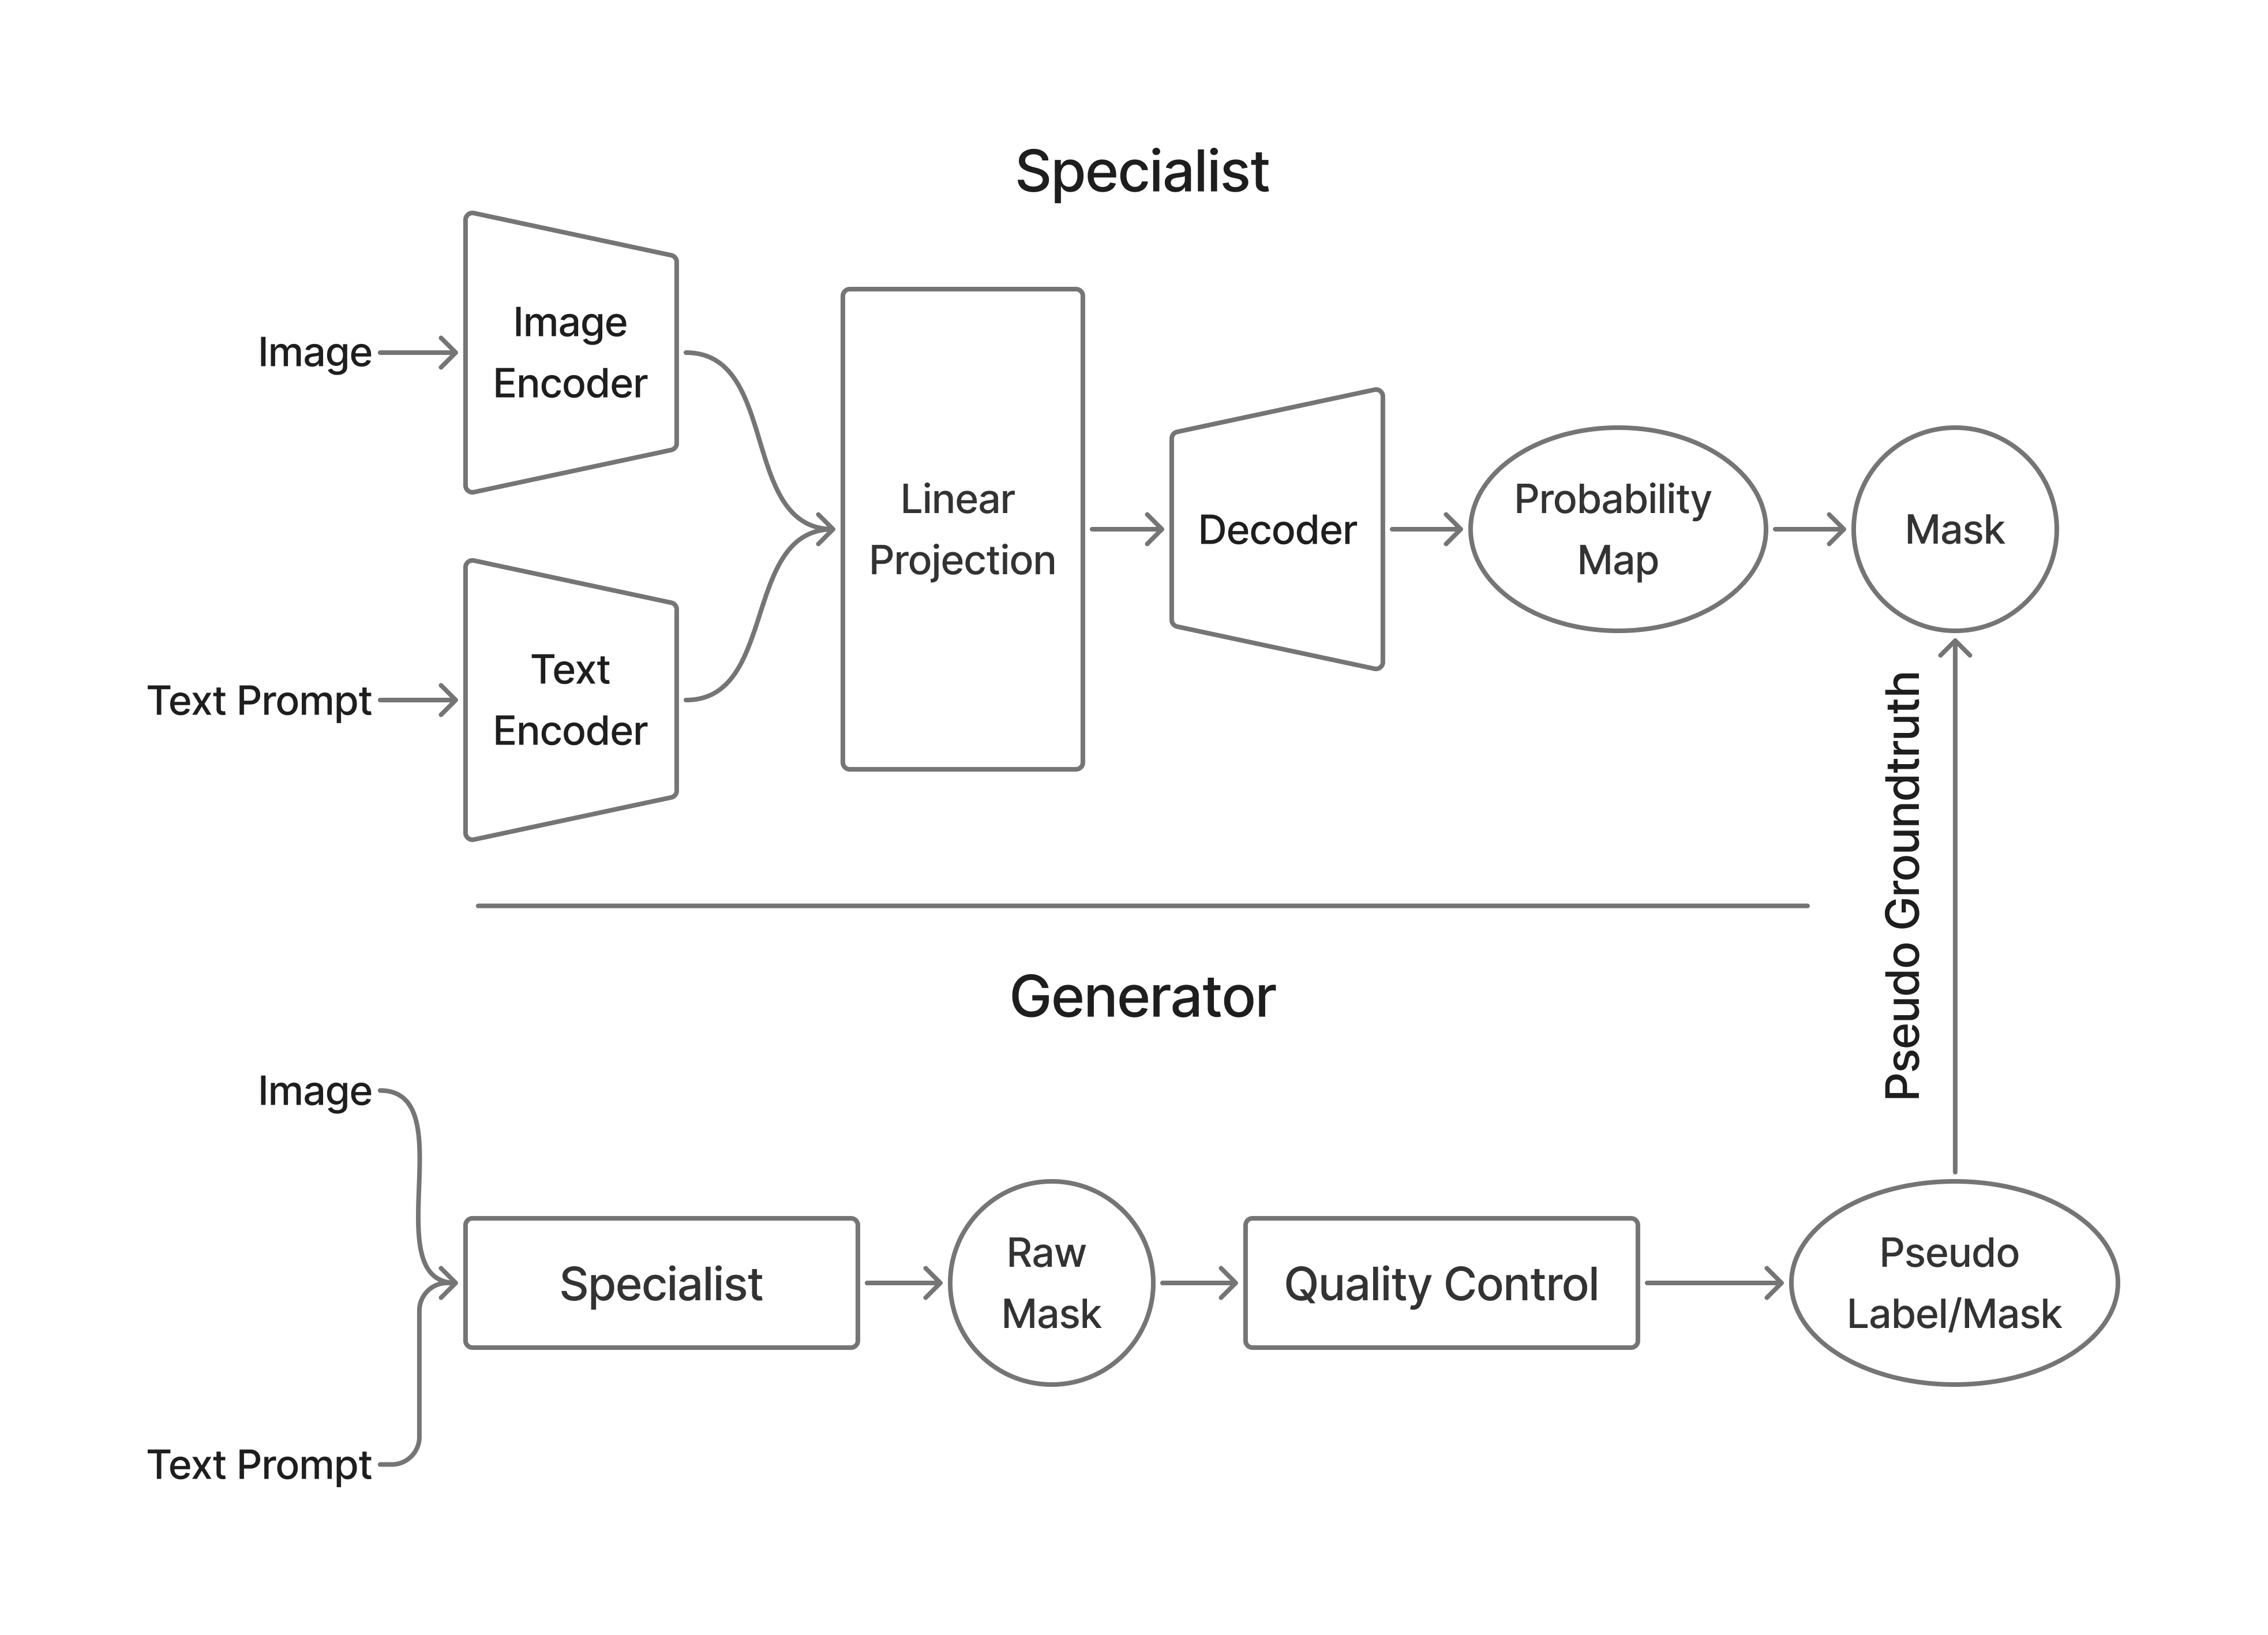
\includegraphics[width=\linewidth]{images/offline-pipeline.png}
        \caption{Pipeline huấn luyện mô hình}
        \label{fig:offline}
    \end{minipage}
    \hfill
    \begin{minipage}{0.48\textwidth}
        \centering
        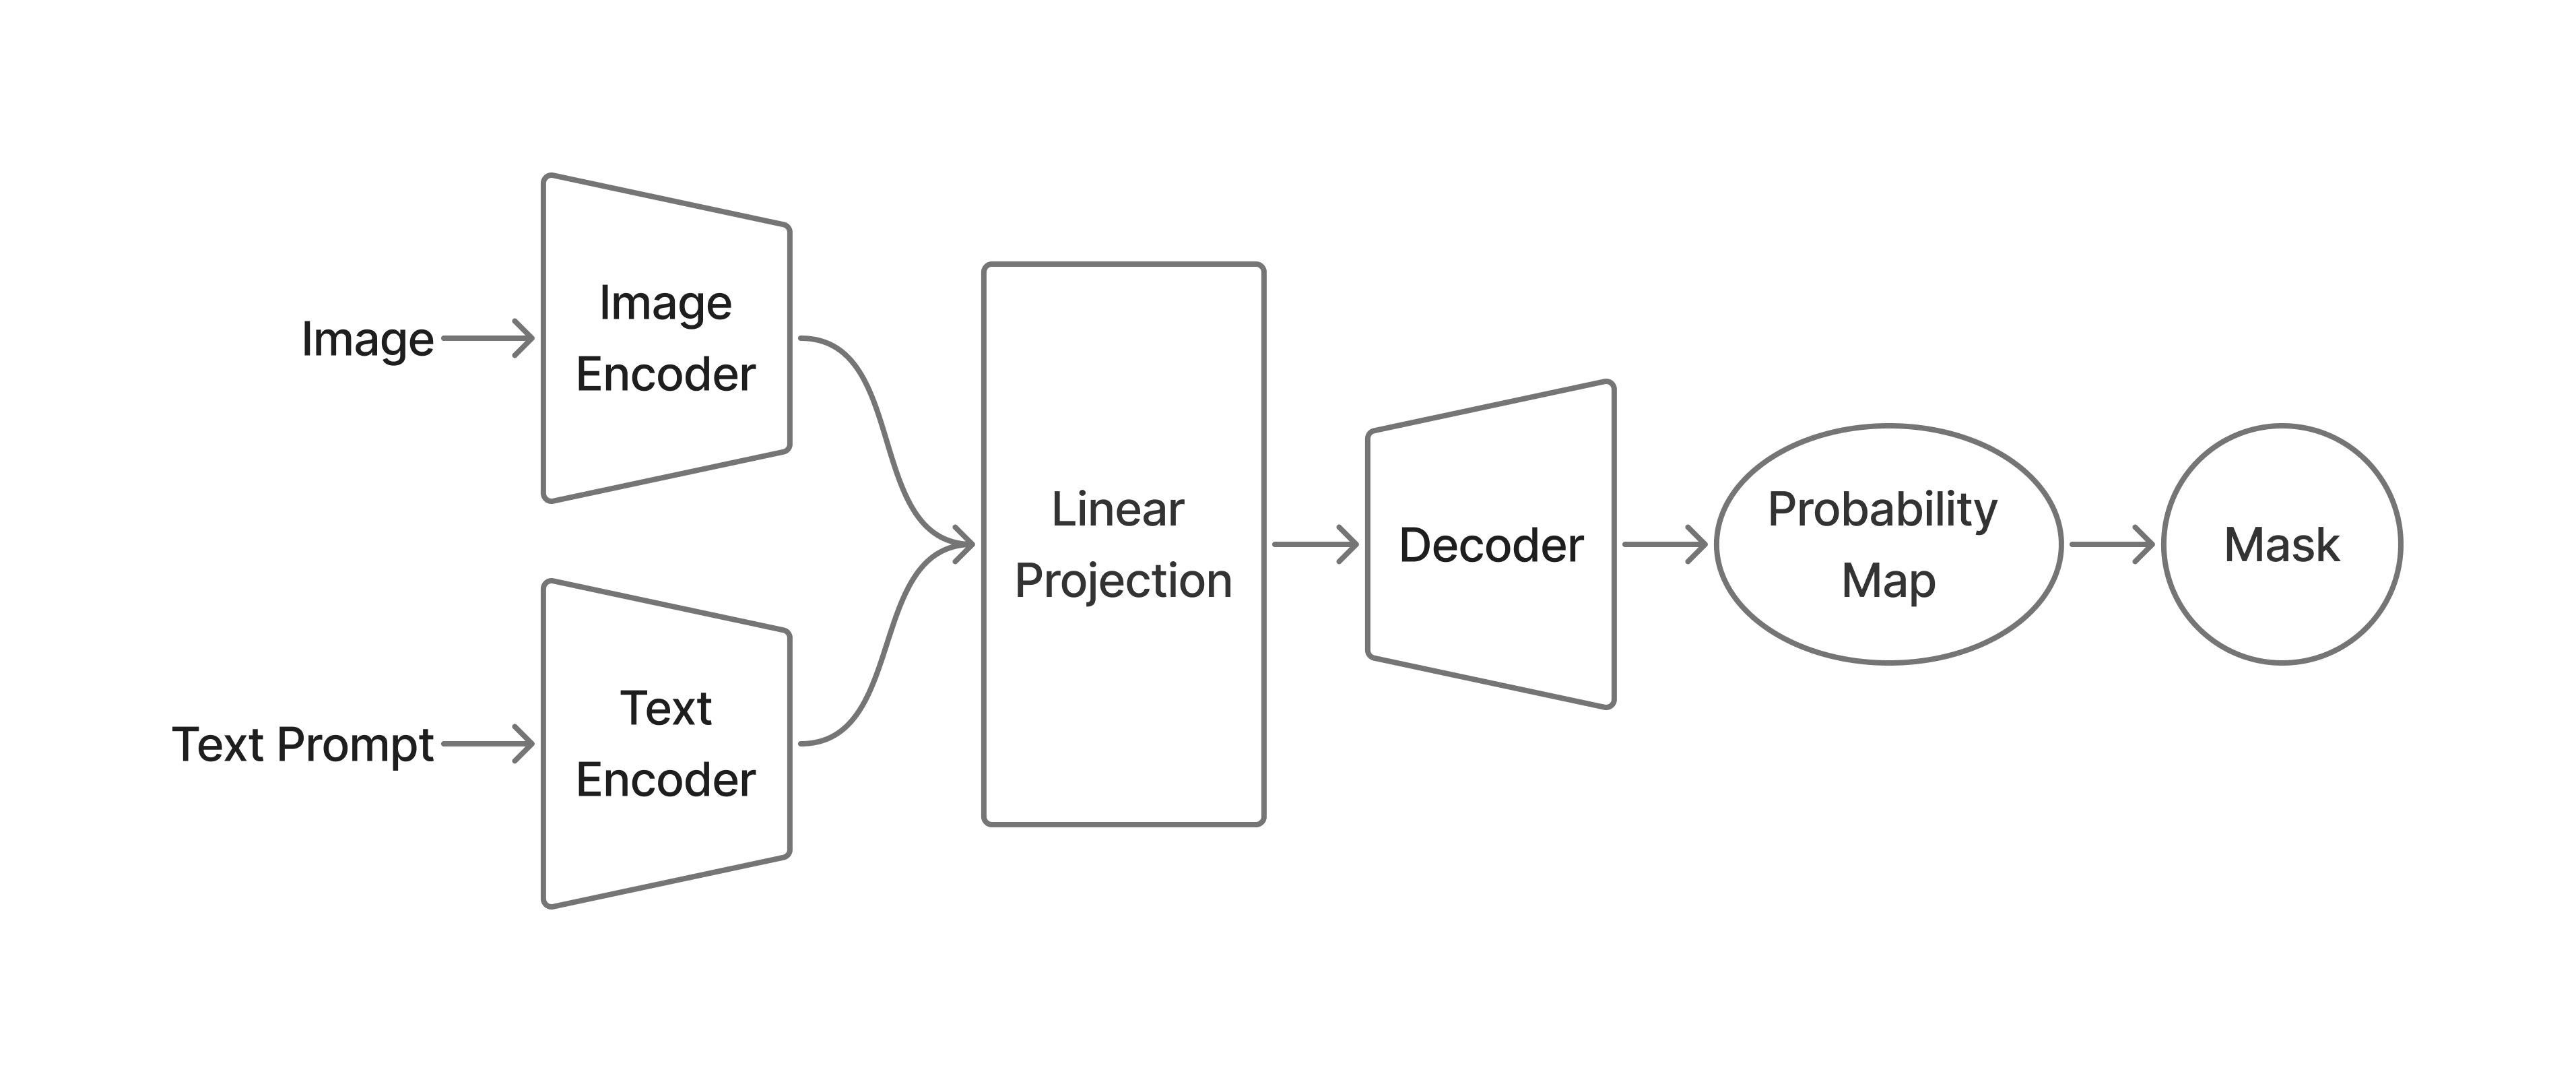
\includegraphics[width=\linewidth]{images/online-pipeline.png}
        \caption{Pipeline sử dụng mô hình}
        \label{fig:online}
    \end{minipage}
\end{figure}

\begin{figure}[H]
    \centering
    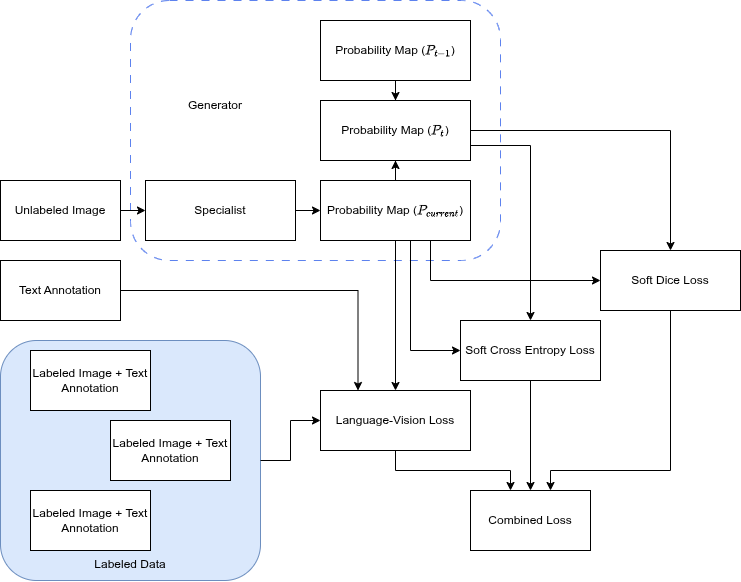
\includegraphics[width=0.8\textwidth]{images/lvit_loss_calculation.png}
    \caption{Pipeline tính toán hàm mất mát và xây dựng nhãn giả chi tiết}
    \label{fig:loss_calculation}
\end{figure}

Hình \ref{fig:offline} mô tả pipeline huấn luyện mô hình ở chế độ ngoại tuyến. Trong giai đoạn này, hệ thống sử dụng cả dữ liệu có nhãn và dữ liệu không nhãn. Đối với dữ liệu có nhãn, mặt nạ chuẩn được dùng trực tiếp để tính các hàm mất mát giám sát như Dice loss và Cross-Entropy. Đối với dữ liệu không nhãn, mô hình cần thêm cơ chế sinh nhãn giả để tạo ra mặt nạ tạm thời phục vụ quá trình huấn luyện. Pipeline này gồm hai thành phần quan trọng: \textit{Specialist} và \textit{Generator}. Specialist chịu trách nhiệm sinh mặt nạ phân đoạn ban đầu dựa trên ảnh đầu vào và câu nhắc văn bản, trong khi Generator tổng hợp và cập nhật các nhãn giả ổn định hơn từ các dự đoán qua nhiều vòng huấn luyện.

Trong pipeline huấn luyện, các bước như \textit{Quality Control}, \textit{Pseudo Groundtruth Generation} và \textit{Loss Calculation} đóng vai trò trung gian quan trọng. Quality Control giúp kiểm soát chất lượng nhãn giả trước khi sử dụng cho huấn luyện. Pseudo Groundtruth Generation cập nhật mặt nạ giả bằng cơ chế EPI/EMA để làm mượt các dự đoán qua thời gian. Loss Calculation kết hợp các thành phần mất mát từ dữ liệu có nhãn, dữ liệu không nhãn và tín hiệu căn chỉnh ngôn ngữ-thị giác. Các bước này không được thiết kế như các mô-đun độc lập, mà được tích hợp vào nhiều giai đoạn khác nhau của quá trình huấn luyện và được trình bày chi tiết hơn trong Hình \ref{fig:loss_calculation}.

Hình \ref{fig:online} mô tả pipeline sử dụng mô hình trong thực tế sau khi quá trình huấn luyện đã hoàn tất. Ở giai đoạn suy luận, người dùng cung cấp một ảnh y khoa và một câu nhắc văn bản mô tả vùng cần phân đoạn. Ảnh được đưa qua nhánh mã hóa thị giác, trong khi câu nhắc được chuyển thành đặc trưng ngữ nghĩa thông qua bộ mã hóa văn bản. Hai nguồn đặc trưng này được kết hợp trong mô hình để sinh ra bản đồ xác suất phân đoạn. Sau đó, bản đồ xác suất được xử lý bằng một ngưỡng quyết định để tạo ra mặt nạ nhị phân cuối cùng. Mặt nạ này biểu diễn vùng tổn thương hoặc cơ quan phù hợp với nội dung câu nhắc đầu vào.

Điểm quan trọng của pipeline online là mô hình có tính linh hoạt theo câu nhắc. Cùng một ảnh đầu vào có thể tạo ra các mặt nạ khác nhau nếu người dùng thay đổi mô tả văn bản. Điều này giúp mô hình phù hợp hơn với các tình huống tương tác trong y khoa, nơi bác sĩ hoặc nhà nghiên cứu có thể muốn tập trung vào một vùng tổn thương, một cơ quan hoặc một đặc điểm bệnh lý cụ thể.

Hình \ref{fig:loss_calculation} mô tả chi tiết quá trình xây dựng nhãn giả và tính toán hàm mất mát cho ảnh không nhãn. Trước hết, mô hình nhận ảnh không nhãn cùng câu nhắc văn bản tương ứng để sinh ra bản đồ xác suất hiện tại $P_{current}$. Mỗi phần tử trong $P_{current}$ biểu diễn xác suất pixel tương ứng thuộc về vùng cần phân đoạn, thay vì chỉ đưa ra quyết định nhị phân là nền hoặc tổn thương. Do đó, $P_{current}$ không chỉ cho biết vị trí vùng dự đoán mà còn thể hiện mức độ tự tin của mô hình tại từng điểm ảnh.

Bản đồ xác suất hiện tại này được kết hợp với nhãn giả ở vòng trước $P_{t-1}$ thông qua cơ chế EPI để tạo ra bản đồ xác suất giả mới $P_t$. Về bản chất, EPI hoạt động như một phép trung bình động theo thời gian: những vùng được mô hình dự đoán nhất quán qua nhiều vòng huấn luyện sẽ được củng cố, trong khi các vùng chỉ xuất hiện do nhiễu hoặc sai số tạm thời sẽ bị làm giảm ảnh hưởng. Nhờ vậy, $P_t$ thường ổn định hơn so với dự đoán đơn lẻ ở vòng hiện tại và có thể được sử dụng như một pseudo groundtruth đáng tin cậy hơn cho quá trình huấn luyện trên dữ liệu không nhãn.

Điểm quan trọng là các hàm mất mát trong bước này được áp dụng theo hướng \textit{soft}. Điều này có nghĩa là mục tiêu huấn luyện không bắt buộc phải là mặt nạ nhị phân chỉ gồm các giá trị 0 và 1, mà có thể là một bản đồ xác suất với các giá trị thực nằm trong khoảng từ 0 đến 1. Ví dụ, một pixel có giá trị 0.8 trong nhãn giả thể hiện rằng pixel đó có khả năng cao thuộc vùng tổn thương, trong khi giá trị 0.4 thể hiện mức độ không chắc chắn lớn hơn. Cách biểu diễn này giữ lại nhiều thông tin hơn so với việc gán cứng pixel đó thành 0 hoặc 1.

Việc sử dụng nhãn mềm đặc biệt phù hợp với phân đoạn ảnh y khoa, vì ranh giới giữa vùng bệnh lý và mô lành thường không rõ ràng tuyệt đối. Trong nhiều trường hợp, các pixel nằm gần biên tổn thương có thể mang thông tin mơ hồ, khiến cả mô hình lẫn chuyên gia chú thích khó đưa ra quyết định hoàn toàn chắc chắn. Nếu áp dụng ngưỡng nhị phân quá sớm trong huấn luyện, các vùng có xác suất trung gian sẽ bị mất thông tin về độ không chắc chắn. Ngược lại, khi giữ nhãn giả ở dạng xác suất, mô hình có thể học được biểu diễn phân đoạn mềm và điều chỉnh dần ranh giới dự đoán qua các vòng tối ưu.

Cách tiếp cận này cũng giúp Dice loss và Cross-Entropy nhận được tín hiệu huấn luyện mượt hơn. Thay vì phạt mô hình theo một nhãn cứng duy nhất, các hàm mất mát có thể so sánh trực tiếp dự đoán của mô hình với phân phối xác suất $P_t$. Điều này làm giảm nguy cơ mô hình học quá mạnh từ các nhãn giả sai ở giai đoạn đầu, đồng thời cho phép các dự đoán có độ tin cậy cao đóng góp nhiều hơn vào quá trình cập nhật tham số. Về mặt ý tưởng, cơ chế này tương tự Knowledge Distillation, trong đó một phân phối mềm được dùng làm mục tiêu để truyền đạt thông tin giàu hơn so với nhãn lớp cố định.

Sau khi có $P_t$, hệ thống sử dụng bản đồ xác suất giả này để tính các hàm mất mát phân đoạn như Dice loss và Cross-Entropy. Đồng thời, bản đồ xác suất ban đầu $P_{current}$ được kết hợp với câu nhắc văn bản đi kèm để tính Language-Vision Loss. Thành phần Language-Vision Loss giúp kiểm tra xem vùng dự đoán có nhất quán với mô tả văn bản hay không, từ đó bổ sung tín hiệu giám sát ngữ nghĩa cho dữ liệu không nhãn. Cuối cùng, các thành phần mất mát này được kết hợp theo trọng số để tạo ra hàm mất mát tổng, dùng để cập nhật tham số của mô hình.

Ba pipeline trong phần này cho thấy LViT không chỉ là một mô hình phân đoạn ảnh thông thường, mà là một hệ thống học đa phương thức có khả năng tận dụng đồng thời ảnh, văn bản, nhãn chuẩn và nhãn giả. Pipeline huấn luyện giúp mô hình học từ cả dữ liệu có nhãn và không nhãn; pipeline online cho phép sử dụng mô hình với câu nhắc văn bản; còn pipeline tính loss mô tả cách các tín hiệu giám sát được kết hợp để cải thiện chất lượng phân đoạn.